\PassOptionsToPackage{}{graphicx}
\documentclass[fullscreen=true, unicode, bookmarks=false]{beamer}

\usepackage{lmodern}
\usepackage[T2A]{fontenc} 
\usepackage[UTF8]{inputenc}
\usepackage[russian]{babel}
\usepackage{amsmath,amsfonts,amssymb}
\usepackage[export]{adjustbox}
\usepackage{textgreek}
\usepackage{epstopdf}
\sloppy

\setbeamertemplate{navigation symbols}{}

\usetheme{Madrid}
\usecolortheme{whale}

\usefonttheme{professionalfonts}

\usepackage{etoolbox}

\newcommand\Pitem{%
  \addtocounter{enumi}{-1}%
  \renewcommand\theenumi{\arabic{enumi}'}%
  \item%
  \renewcommand\theenumi{\arabic{enumi}}%
}
\setbeamertemplate{enumerate item}[square]

\makeatletter
\newcommand\titlegraphicii[1]{\def\inserttitlegraphicii{#1}}
\titlegraphicii{}
\setbeamertemplate{title page}
{
    \begin{centering}
    \begin{beamercolorbox}[sep=8pt,center]{institute}
      \usebeamerfont{institute}\insertinstitute
    \end{beamercolorbox}
    \vspace{0.25cm}
    \begin{beamercolorbox}[sep=8pt,center]{title}
      \usebeamerfont{title}\inserttitle\par%
      \ifx\insertsubtitle\@empty%
      \else%
        \vskip0.25em%
        {\usebeamerfont{subtitle}\usebeamercolor[fg]{subtitle}\insertsubtitle\par}%
      \fi%     
    \end{beamercolorbox}%
    \vskip1em\par
    \begin{beamercolorbox}[sep=8pt,center]{author}
      \usebeamerfont{author}\insertauthor
    \end{beamercolorbox}
  \end{centering}
}
\makeatother
\title[]{{\huge Бифуркационные особенности одного класса краевых задач параболического типа со специальными краевыми условиями}}
\date{}
\institute[]{Федеральное государственное бюджетное образовательное \\
учреждение высшего образования \\
«Ярославский государственный университет им. П.Г.Демидова»
}

\begin{document}

\begin{frame}[plain]
\maketitle
\small
\begin{tabular}[t]{@{}l@{\hspace{3pt}}p{.29\textwidth}@{}}
Аспирант: & \\
Ивановский Л.И.
\end{tabular}%
\small
\begin{tabular}[t]{@{}l@{\hspace{3pt}}p{.3\textwidth}@{}}
Научный руководитель: & \\
д. ф.-м.н., профессор Глызин С.Д.
\end{tabular}%
\end{frame}

\begin{frame}
\frametitle{ Объекты и цели исследования }

\begin{block}{}
Объектами исследования являются устойчивые режимы динамических систем
\end{block}

\vfill

\begin{block}{}
Цель исследования заключается в изучении поведения устойчивых режимов системы дифференциальных уравнений с импульсными воздействиями и краевой задачи со специальными краевыми условиями
\end{block}

\end{frame}

\begin{frame}
\frametitle{ Задачи исследования }

\begin{itemize}
\item Для нелинейной динамической системы с импульсными воздействиями выделить области с разными бифуркационными сценариями, и изучить перестройки, происходящие в фазовом пространстве модельного отображения.

\vfill

\item Для краевой задачи со специальными краевыми условиями выявить критические зависимости параметров, при которых происходит потеря устойчивости нулевого решения. При значениях параметров, близких к критическим, определить условия появления неоднородных состояний равновесия и циклов.
\end{itemize}

\end{frame}

\begin{frame}
\frametitle{ Положения, выносимые на публичное представление }

\begin{enumerate}
\begin{small}
\item Области с разными бифуркационными сценариями в случае цепочки и кольца осцилляторов с диффузионным взаимодействием и кольца однонаправленно связанных осцилляторов.
\item Перестройки, происходящие в фазовом пространстве модельного отображения динамической системы с импульсными воздействиями.
\item Критические зависимости параметров, при которых происходит потеря устойчивости нулевого решения краевой задачи со специальными краевыми условиями.
\item Уравнения амплитуды колебаний нулевого состояния равновесия в случае дивергентной и колебательной потери устойчивости.
\end{small}
\end{enumerate}

\end{frame}

\begin{frame}
\frametitle{ Система связанных осцилляторов }

\begin{eqnarray}\label{u_system} 
	\dot{u_j} = d(a_1u_{j-1}-a_2u_j+u_{j+1})+\lambda[-1+\alpha f(u_j(t-1)) - \beta g(u_j)]u_j, \nonumber \\ j=\overline{1,m},
\end{eqnarray}		

$$ a_1, a_2 \in \{0, 1, 2\}, \quad d , \beta \in \mathbb{R}_+, \quad \lambda >> 1, \quad \alpha > 1 + \beta; $$
$$ u_j=u_j(t)>0, \quad f(u), g(u) \in C^2(\mathbb{R}_+), $$
$$ f(0) = g(0) = 1, \quad 0 < \beta g(u) < \alpha, \quad \forall u \in \mathbb{R}_+; $$
$$ f(u), g(u), uf'(u), ug'(u), u^2f''(u), u^2g''(u) = O(1/u), \; u \to +\infty. $$

\vfill

\begin{itemize}
\item { $ a_1 = 1, \, a_2 = 2; \quad u_0=u_1, \, u_3=u_4. $ }
\item { $ a_1 = 1, \, a_2 = 2; \quad u_0=u_3, \, u_1=u_4. $ }
\item { $ a_1 = 0, \, a_2 = 1; \quad u_1=u_4. $ }
\end{itemize}

\end{frame}

\begin{frame}

$$ u_1 \equiv u_2 \equiv \ldots \equiv u_m = u_*(t, \lambda) $$
$$ \dot{u} = \lambda(-1+\alpha f(u(t-1)) - \beta g(u))u $$
$$ T_*(\lambda): \quad \lim_{\lambda\to\infty} T_*(\lambda) = T_0 = \alpha + 1 + (\beta+1)/(\alpha - \beta - 1). $$

\vfill

$$ u_1 = \mbox{exp} \left( \frac{x}{\varepsilon} \right), \quad \varepsilon = \frac{1}{\lambda} << 1, $$
$$ u_j = \mbox{exp} \left( \frac{x}{\varepsilon} + \sum\limits_{k=1}^{j-1} y_k \right), \quad j = \overline{2,m}, $$ 
$$ \dot{x} = -1 + \alpha f \left( \mbox{exp} \, \left( \frac{x(t-1)}{\varepsilon} \right) \right) - \beta g \left( \mbox{exp} \, \left( \frac{x}{\varepsilon} \right) \right). $$

\end{frame}

\begin{frame}
\frametitle{Система с импульсными воздействиями} 

\begin{eqnarray}\label{y_system}
\dot{y_1} = d(e^{y_{j+1}} + a_1\,e^{-y_j} - e^{y_j} - a_1\,e^{y_{j-1}}), \quad  j=\overline{1,m-1},
\end{eqnarray}

$$ y_j(+0) = \frac{\alpha -1}{\alpha - \beta - 1}y_j(-0), $$
$$ y_j(1+0) = y_j(1-0) - \frac{\alpha}{\alpha - 1}y_j(+0), $$
$$ y_j(\alpha + 0) = (1 + \beta)y_j(\alpha - 0), $$
$$ y_j(\alpha + 1 + 0) = y_j(\alpha + 1 - 0) - \frac{\alpha}{1 + \beta}y_j(\alpha + 0). $$

\begin{itemize}
\item { $ y_0 = y_3 = 0 $ }
\item { $ y_0 = y_3 = -(y_1 + y_2) $ }
\item { $ y_3 = -(y_1 + y_2) $ }
\end{itemize}

\end{frame}

\begin{frame}
\frametitle{Модельное отображение} 

\begin{equation}\label{phi_z} 
	\Phi(z): \begin{pmatrix}
           z_1 \\
           z_2
          \end{pmatrix}
					\to
					\begin{pmatrix}
           y_1(T_0, z_1, z_2) \\
           y_2(T_0, z_1, z_2)
          \end{pmatrix},
\end{equation}

$$ y_1(-0, z_1, z_2) = z_1, \quad y_2(-0, z_1, z_2) = z_2 $$

\vfill

\begin{block}{Теорема} 
Любой грубой неподвижной точке $ z $ отображения \eqref{phi_z}, в системе \eqref{y_system} и как следствие в системе \eqref{u_system}, соответствует цикл периода $ T_0 $ с теми же свойствами устойчивости.
\end{block} 

\end{frame}

\begin{frame}
\frametitle{Области параметров, соответствующие различным бифуркационным сценариям }

\begin{figure}[h]
\hspace{-1.5cm}
\begin{minipage}[h]{0.2\linewidth}
\center{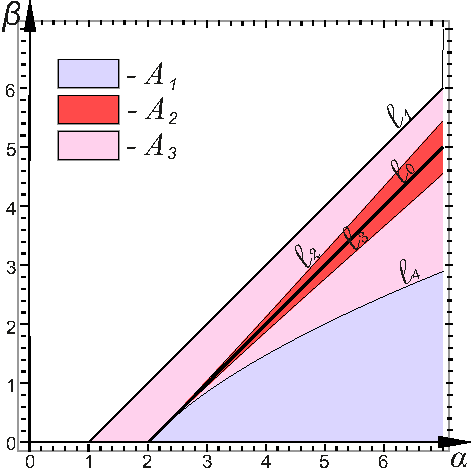
\includegraphics[scale=0.47]{chain.pdf} \\ a) }
\end{minipage}
\hspace{1.5cm}
\begin{minipage}[h]{0.2\linewidth}
\center{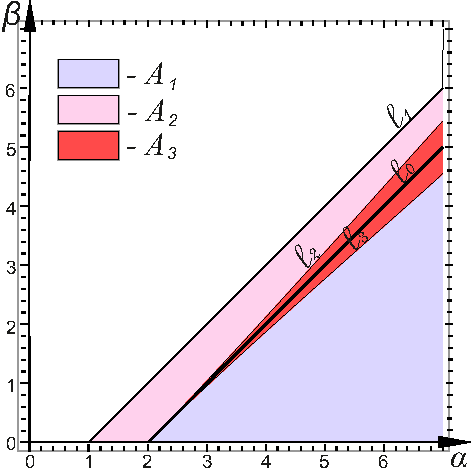
\includegraphics[scale=0.47]{ring.pdf} \\ b) }
\end{minipage}
\hspace{1.5cm}
\begin{minipage}[h]{0.2\linewidth}
\center{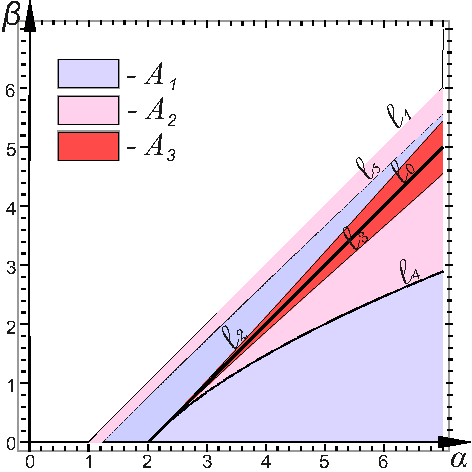
\includegraphics[scale=0.47]{wave.pdf} \\ c) }
\end{minipage}
\end{figure}

\end{frame}

\begin{frame}
\frametitle{Случай цепочки связанных осцилляторов}

\begin{figure}[h]
\hspace{-1.5cm}
\begin{minipage}[h]{0.2\linewidth}
\center{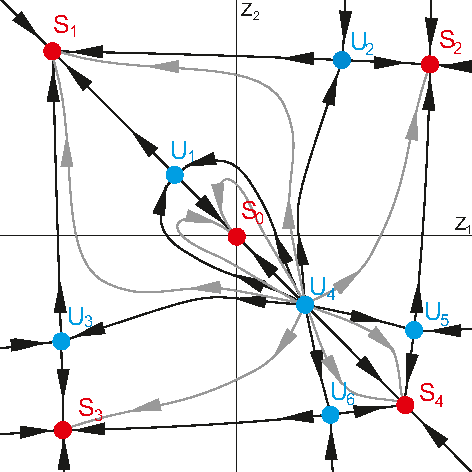
\includegraphics[scale=0.47]{2a.pdf}  \\ a) $ (\alpha, \beta) \in A_1 $ }
\end{minipage}
\hspace{1.5cm}
\begin{minipage}[h]{0.2\linewidth}
\center{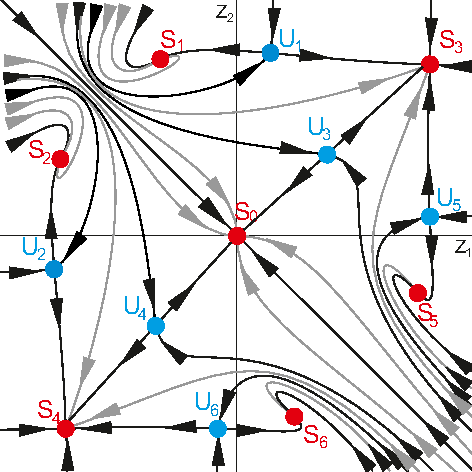
\includegraphics[scale=0.47]{5a.pdf}  \\ b) $ (\alpha, \beta) \in A_2 $ }
\end{minipage}
\hspace{1.5cm}
\begin{minipage}[h]{0.2\linewidth}
\center{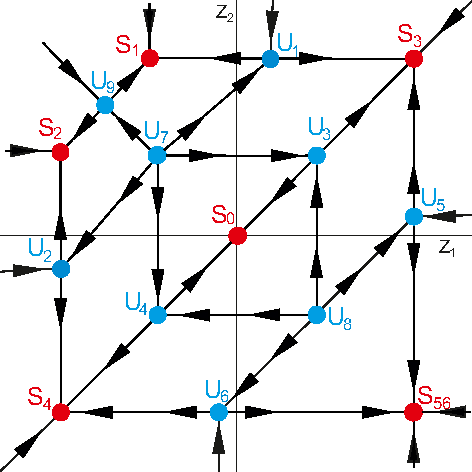
\includegraphics[scale=0.47]{6b.pdf}  \\ c) $ (\alpha, \beta) \in A_3 $ }
\end{minipage}
\end{figure}

\end{frame}

\begin{frame}
\frametitle{Случай кольца осцилляторов с диффузионным взаимодействием}

\begin{figure}[h]
\hspace{-1.5cm}
\begin{minipage}[h]{0.2\linewidth}
\center{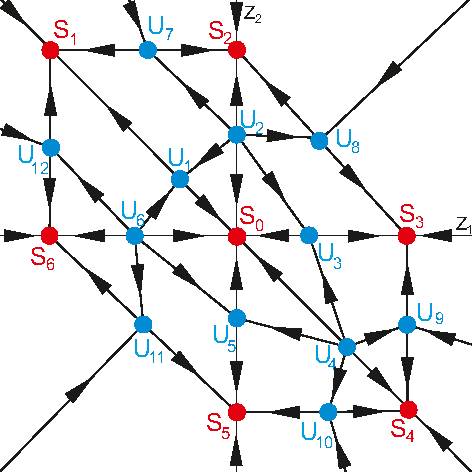
\includegraphics[scale=0.47]{11a.pdf}  \\ a) $ (\alpha, \beta) \in A_1 $ }
\end{minipage}
\hspace{1.5cm}
\begin{minipage}[h]{0.2\linewidth}
\center{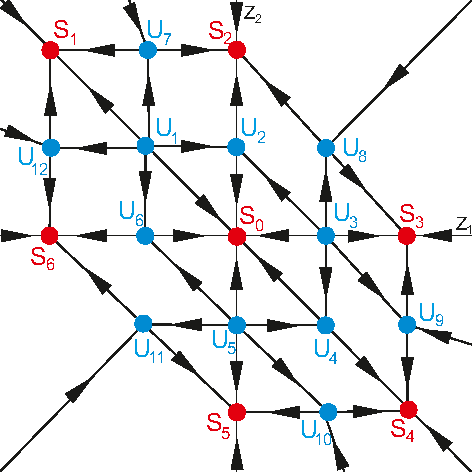
\includegraphics[scale=0.47]{13a.pdf}  \\ b) $ (\alpha, \beta) \in A_2 $ }
\end{minipage}
\hspace{1.5cm}
\begin{minipage}[h]{0.2\linewidth}
\center{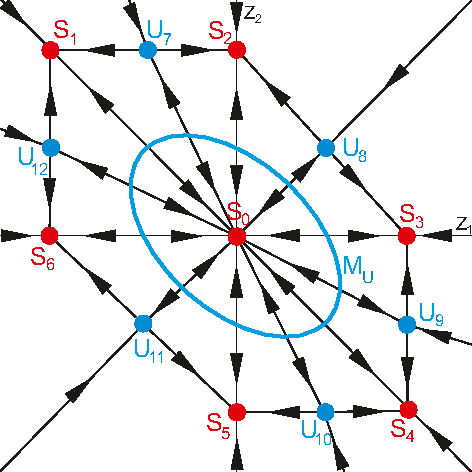
\includegraphics[scale=0.47]{15.pdf}  \\ c) $ (\alpha, \beta) \in A_3 $ }
\end{minipage}
\end{figure}

\end{frame}

\begin{frame}
\frametitle{Случай кольца однонаправленно связанных осцилляторов}

\begin{figure}[h]
\hspace{-1.5cm}
\begin{minipage}[h]{0.2\linewidth}
\center{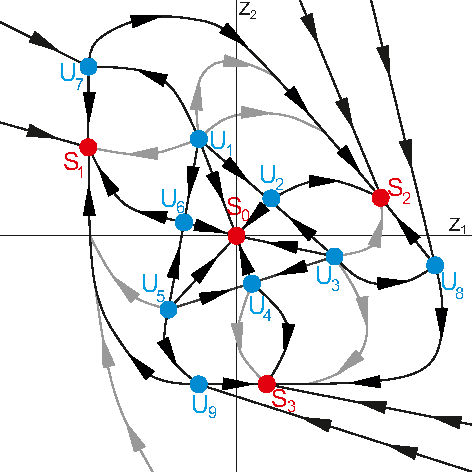
\includegraphics[scale=0.47]{17a.pdf}  \\ a) $ (\alpha, \beta) \in A_1 $ }
\end{minipage}
\hspace{1.5cm}
\begin{minipage}[h]{0.2\linewidth}
\center{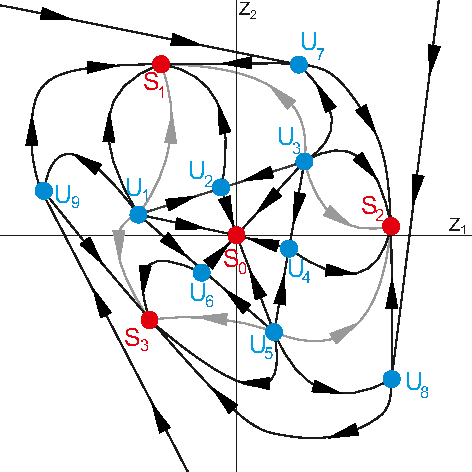
\includegraphics[scale=0.47]{18a.pdf}  \\ b) $ (\alpha, \beta) \in A_2 $ }
\end{minipage}
\hspace{1.5cm}
\begin{minipage}[h]{0.2\linewidth}
\center{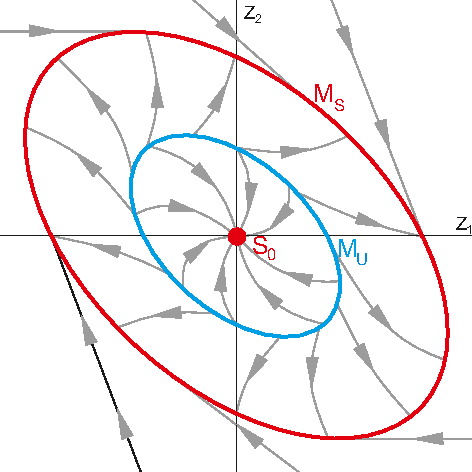
\includegraphics[scale=0.47]{20b.pdf}  \\ c) $ (\alpha, \beta) \in A_3 $ }
\end{minipage}
\end{figure}

\end{frame}

\begin{frame}
\frametitle{ Краевая задача с отклонением в краевом условии }

\begin{equation}\label{boundary_problem}
	\dot u = u'' + \gamma u - \delta u^3,	
\end{equation}

\begin{equation}\label{boundary_cond}	
	u'(0, t) \, = 0, \qquad u'(1, t) \, = F(u)
\end{equation}

$$ t \geqslant 0, \quad x \in [0,1], \quad \delta \in \{0, 1\}, \quad \gamma \in \mathbb{R}. $$

\vfill

\begin{itemize}

\item $ F(u) = \alpha\,u(x_0, t), \; \delta=1; \quad \alpha \in \mathbb{R}, \; x_0 \in [0, 1). $
\item $ F(u) \, = \alpha\,u(x_0, t) + \beta u^3(x_0, t), \; \delta=0; \quad \beta \in \mathbb{R}. $
\item $ F(u) \, = \alpha\int\limits_{0}^{1} u(y, t) dy, \; \delta = 1. $

\end{itemize}

\end{frame}

\begin{frame}
\frametitle{ Линеаризованная краевая задача }
 
\begin{equation}
	\dot u = u'' + \gamma u,	
\end{equation}

\vfill

$$ u'(0, t) \, = 0, $$

\vfill

\begin{itemize}

\item $ u'(1, t) \, = \alpha\,u(x_0, t). $
\item $ u'(1, t) \, = \alpha\int\limits_{0}^{1} u(y, t) dy. $

\end{itemize}

\end{frame}

\begin{frame}
\frametitle{ Задача на собственные значения }
 
$$ u(x, t) = e^{\lambda t} \, v(x). $$

\bigskip
 
\begin{equation} 
	v'' + (\gamma - \lambda)v = 0,
\end{equation}

\vfill
	
$$ v'(0) \, = 0, $$

\vfill

\begin{itemize}

\item $ v'(1) \, = \alpha\,v(x_0). $
\item $ v'(1) \, = \alpha\int\limits_{0}^{1} v(y) dy. $

\end{itemize}

\vfill

$$ v(x) = c \ch  \mu x, \quad c \in \mathbb{R}, \, \mu = \sqrt{-\gamma + \lambda}. $$

\end{frame}

\begin{frame}
\frametitle{ Потеря устойчивости нулевого состояния равновесия }

\begin{itemize}

\item { $ \lambda = 0: \; \mu = \sqrt{-\gamma}, $ 
}

\begin{equation}
\alpha_u = \left\{
                \begin{array}{ll}
                  -\gamma, \; \mbox{при} \, F(u) \, = \alpha\int\limits_{0}^{1} u(t, y) dy, \\
                  \dfrac{ \sqrt{-\gamma} \, \sh \sqrt{-\gamma} }{ \ch \sqrt{-\gamma} x_0 }, \; \mbox{иначе}.
                \end{array}
              \right.
\end{equation}

\vfill

\item { $ \lambda = i \omega: \; \mu = \sqrt{-\gamma + i \omega}, $ 
}

\begin{equation}
	\alpha_c = \frac{ \sqrt{-\gamma + i \omega} \, \sh \sqrt{-\gamma + i \omega} }{ \ch \sqrt{-\gamma + i \omega} x_0 }.
\end{equation}

\end{itemize}	

\end{frame}

\begin{frame}
\frametitle{ Моделирование линейной краевой задачи }

\begin{equation}\label{numeric_problem} 
	\dot{u}_j =  n^2(u_{j+1} - 2u_j + u_{j-1}) + \gamma u_j, \quad j = \overline{1, n}, 
\end{equation}

\vfill

$$ u_0 = u_1, $$

\vfill

\begin{itemize}

\item $ u_{n+1} = u_n + \frac{\alpha}{n}\:u_k, \quad k \in [1,n]. $
\item $ u_{n+1} = u_n + \frac{\alpha}{n^2} \sum_{k=1}^{n} \:u_k. $

\end{itemize}

\end{frame}

\begin{frame}
\frametitle{ Схематическая визуализация кривых $ \alpha_u $ и $ \alpha_c $ }

\begin{figure}[h]
\hspace{-3.5cm}
\begin{minipage}[h]{0.2\linewidth}
\center{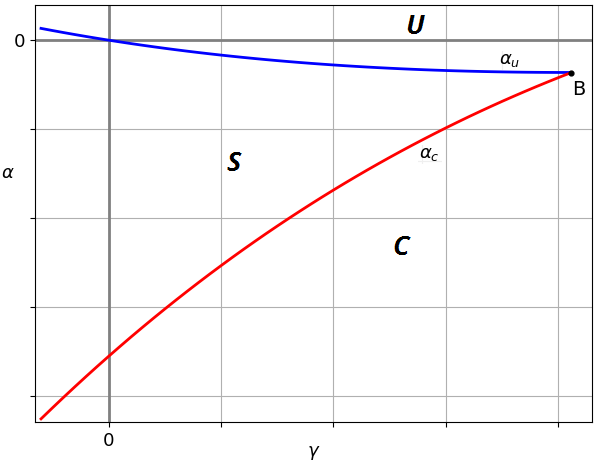
\includegraphics[scale=0.36]{scheme.png} }
\end{minipage}
\hspace{3.5cm}
\begin{minipage}[h]{0.2\linewidth}
\center{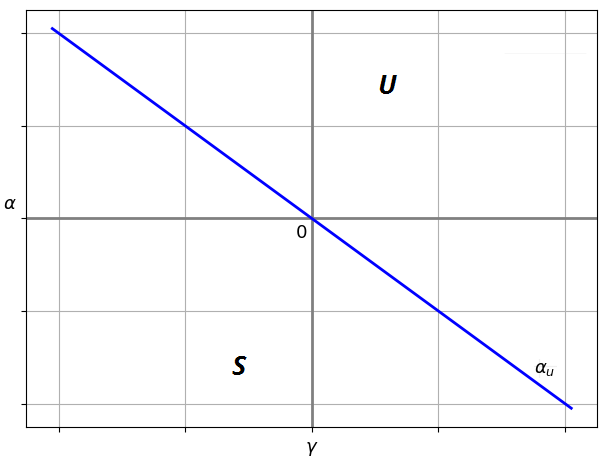
\includegraphics[scale=0.36]{alpha_u.png} }
\end{minipage}
\end{figure}

\end{frame}

\begin{frame}
\frametitle{ Локальный анализ краевой задачи }

\begin{equation}
	u = \sqrt{\varepsilon}u_0 + \varepsilon u_1 + \varepsilon^{\frac{3}{2}} u_2 + O(\varepsilon^2),
\end{equation}

$$ \varepsilon = | \alpha - \alpha_{cr} |, \quad \varepsilon \ll 1, \quad s = \varepsilon t. $$

\vfill

\begin{equation}\label{u_0}
u_0 = u_0'' + \gamma u_0
\end{equation}

\begin{equation}\label{u_2}
\dot u_2 + \frac{\partial u_0}{\partial s} = u_2'' + \gamma u_2 - \delta u_0^3,
\end{equation}

$$ u_0'(0, t) = 0, \quad u_2'(0, t) = 0. $$

\end{frame}

\begin{frame}
\frametitle { Случай дивергентной потери устойчивости }

$$ \lambda = 0: \quad \varepsilon = \alpha - \alpha_u, $$

$$ u_0 = \rho(s) \ch \sqrt{-\gamma} x. $$
\vfill
\begin{itemize}
\item $ u_0'(1, t) = \alpha_u u_0(x_0, t), \; u_2'(1, t) = \alpha_u u_2(x_0, t) + u_0(x_0, t). $
\item $ u_0'(1, t) = \alpha_u u_0(x_0, t), \; u_2'(1, t) = \alpha_u u_2(x_0, t) + u_0(x_0, t). + \beta u_0^3(x_0, t). $
\item $ u_0'(1, t) = \alpha_u\int\limits_{0}^{1} u_0(s, y) dy, \; u_2'(1, t) = \alpha_u\int\limits_{0}^{1} u_2(t, y) dy \, + \, \int\limits_{0}^{1} u_0(s, y) dy. $
\end{itemize}
\vfill
\begin{equation}\label{ro_equation}
	\rho' = \phi_0 \rho + d_0 \rho^3,
\end{equation}
\vfill
$$ u = \pm \sqrt{ \varepsilon \left|\dfrac{\phi_0}{d_0}\right| } \, \ch \sqrt{-\gamma} x + O(\varepsilon). $$
\end{frame}

\begin{frame}
\frametitle {Случай нелинейной краевой задачи с линейным отклонением }

$$ \phi_0 = \frac{ 2 \mu \ch \mu x_0 }{ \mu \ch \mu +\sh \mu - \alpha_u x_0 \sh \mu x_0 }, $$

$$ d_0 = \frac{ -3\gamma \sh 3\mu - 12 \sh \mu - 12 \mu \ch \mu - \alpha_u \mu \ch 3\mu x_0 + 12 \alpha_u x_0 \sh \mu x_0 }{ 16( \sh \mu + \mu \ch \mu - \alpha_u x_0 \sh \mu x_0 ) }. $$

\end{frame}

\begin{frame}
\frametitle { Графики $ \phi_0(\gamma), \; d_0(\gamma) $ }

\begin{figure}[h]
\hspace{-4cm}
\begin{minipage}[h]{0.2\linewidth}
\center{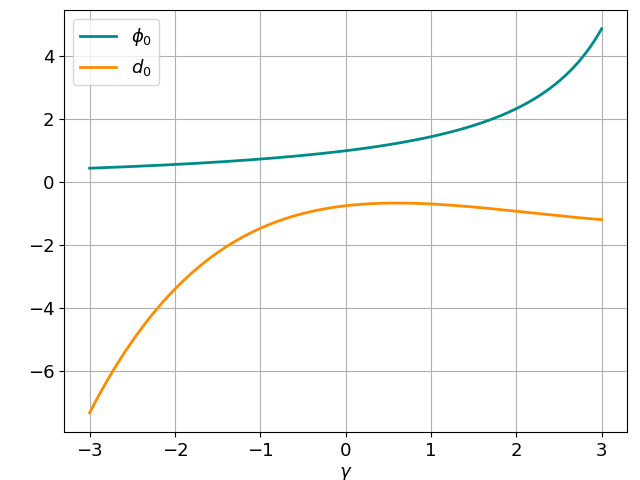
\includegraphics[scale=0.37]{divergent_phi0d0_0.png} \\ a) }
\end{minipage}
\hspace{3.5cm}
\begin{minipage}[h]{0.2\linewidth}
\center{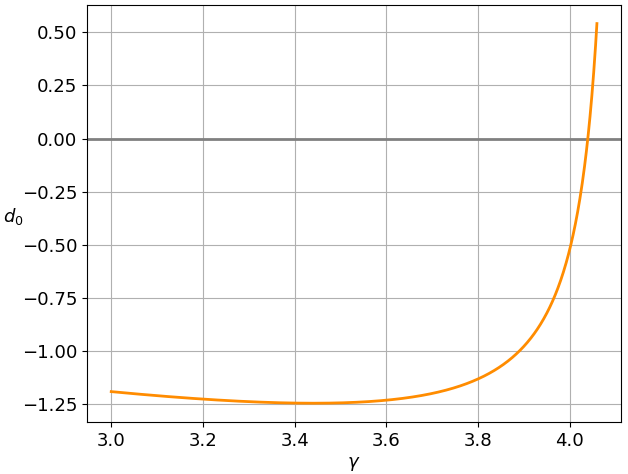
\includegraphics[scale=0.37]{divergent_d0_0.png} \\ b) }
\end{minipage}
\end{figure}

$$ x_0=0 $$

\end{frame}

\begin{frame}
\frametitle { Графики $ \phi_0(\gamma), \; d_0(\gamma) $ }

\begin{center}
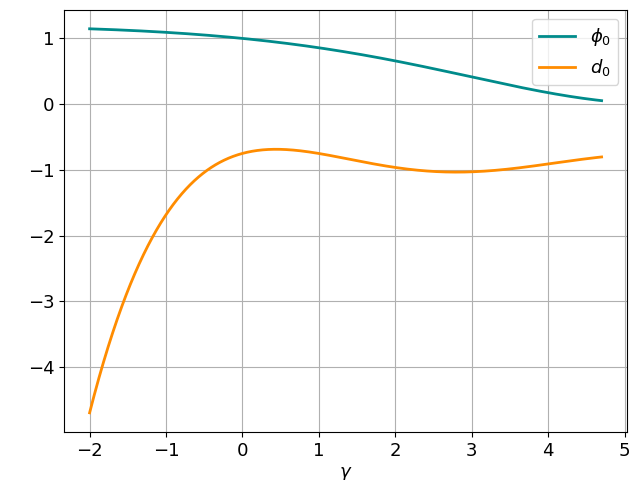
\includegraphics[scale=0.53]{divergent_phi0d0_23.png}
\end{center}

$$ x_0=0.67 $$

\end{frame}

\begin{frame}
\frametitle {Случай линейной краевой задачи с нелинейным отклонением }

$$ \phi_0 = Q \ch \sqrt{-\gamma} x_0, \qquad d_0 = Q \beta \ch^3 \sqrt{-\gamma} x_0, $$

$$ Q = \frac{2 \sqrt{-\gamma}}{\sqrt{-\gamma} \ch \sqrt{-\gamma} + \sh \sqrt{-\gamma} - \alpha_u x_0 \sh \sqrt{-\gamma} x_0}. $$

\end{frame}

\begin{frame}
\frametitle { Графики $ \phi_0(\gamma), \; d_0(\gamma) $ }

\begin{figure}[h]
\hspace{-4cm}
\begin{minipage}[h]{0.2\linewidth}
\center{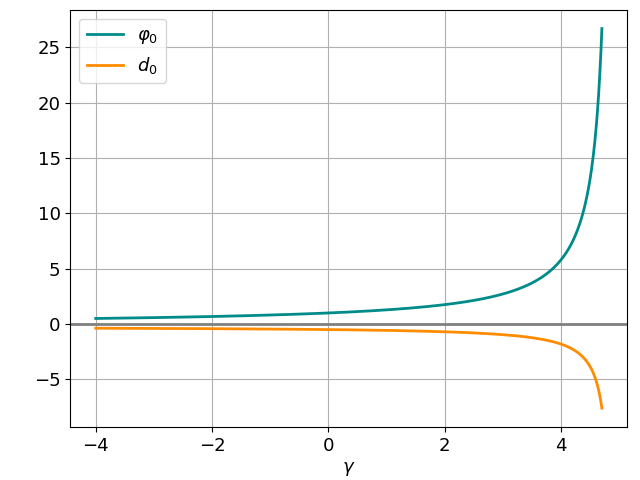
\includegraphics[scale=0.38]{divergent_phi0d0_13_beta_minus.png} \\ a) $\beta = -0.5$ }
\end{minipage}
\hspace{3.7cm}
\begin{minipage}[h]{0.2\linewidth}
\center{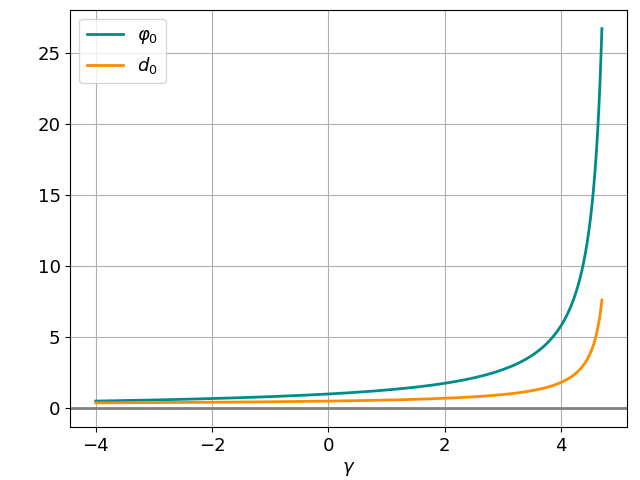
\includegraphics[scale=0.38]{divergent_phi0d0_13_beta_plus.png} \\ b) $\beta = 0.5$ }
\end{minipage}
\end{figure}

$$ x_0=0.33 $$

\end{frame}

\begin{frame}
\frametitle { Графики $ \phi_0(\gamma), \; d_0(\gamma) $ }

\begin{figure}[h]
\hspace{-4cm}
\begin{minipage}[h]{0.2\linewidth}
\center{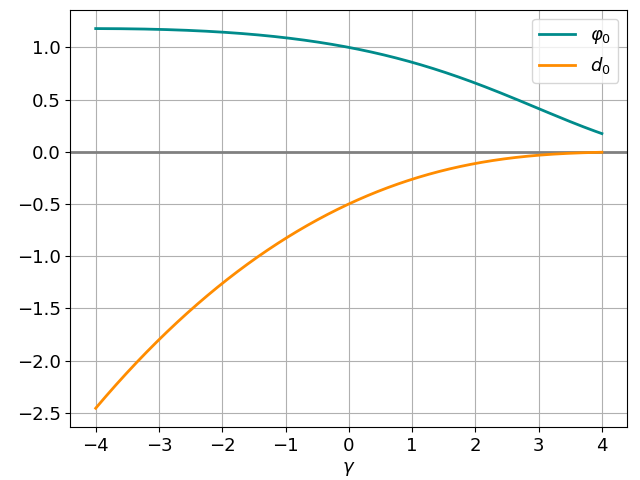
\includegraphics[scale=0.38]{divergent_phi0d0_23_beta_minus.png} \\ a) $\beta = -0.5$ }
\end{minipage}
\hspace{3.7cm}
\begin{minipage}[h]{0.2\linewidth}
\center{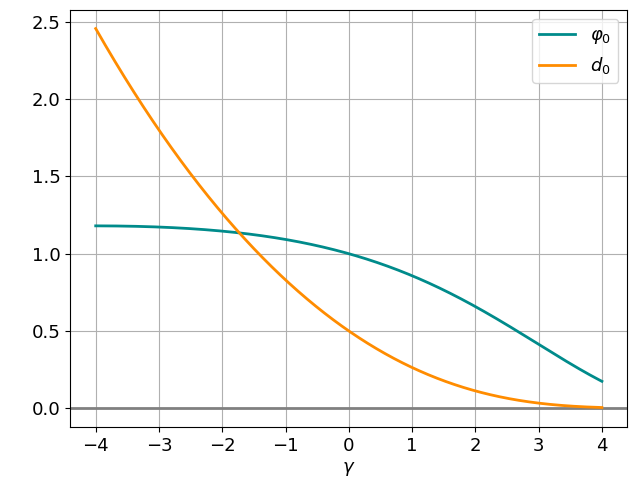
\includegraphics[scale=0.38]{divergent_phi0d0_23_beta_plus.png} \\ b) $\beta = 0.5$ }
\end{minipage}
\end{figure}

$$ x_0=0.67 $$

\end{frame}

\begin{frame}
\frametitle {Случай нелинейной краевой задачи с с интегральным отклонением }

$$ \phi_0 = 1, \qquad d_0 = -\frac{5\gamma\sh3\sqrt{-\gamma}}{48\sh\sqrt{-\gamma}} - \frac{3}{4}. $$

\begin{center}
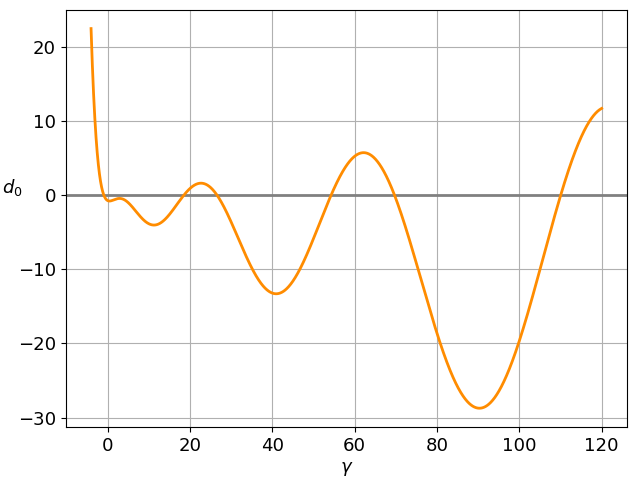
\includegraphics[scale=0.45]{integral_divergent_d0.png}
\end{center}

\end{frame}

\begin{frame}
\frametitle { Случай колебательной потери устойчивости }

$$ \lambda = i\omega: \quad \varepsilon = \alpha_c - \alpha, $$
\vfill
$$ u_0 = z(s) e^{i \omega t} \ch \mu x + \overline{z(s)} e^{-i \omega t} \overline{\ch \mu x}. $$
\vfill
$$ u_0'(1, t) = \alpha_c u_0(x_0, t), $$
\begin{itemize}
\item $ u_2'(1, t) = \alpha_c u_2(x_0, t) + u_0(x_0, t). $
\item $ u_2'(1, t) = \alpha_c u_2(x_0, t) + u_0(x_0, t) + \beta u_0^3(x_0, t). $
\end{itemize}

\begin{equation}\label{z_equation}
	z' = \phi_0 z + d_0 z |z|^2,
\end{equation}

$$ u = \pm \sqrt{ - \varepsilon \dfrac{\phi_0}{d_0} } \, \ch \sqrt{-\gamma + i\omega} x + O(\varepsilon). $$

\end{frame}

\begin{frame}
\frametitle {Случай нелинейной краевой задачи с линейным отклонением }

$$ \phi_0 = \operatorname{Re} \left( \frac{ 2 \mu \ch \mu x_0 }{ \mu \ch \mu +\sh \mu - \alpha_c x_0 \sh \mu x_0 } \right), $$

$$ d_0 = \operatorname{Re} \left( \frac{ 3 \mu ( G(\mu + 2\,\mbox{Re}\mu) + G(\mu + 2i\,\mbox{Im}\mu) + 2G(\overline{\mu}) ) }{ 2 ( \mu \ch \mu +\sh \mu - \alpha_c x_0 \sh \mu x_0 ) } \right), $$

$$ G(y) = \frac{ \alpha_c - y\,\sh y }{ y^2 + \gamma - i\omega }. $$

\end{frame}

\begin{frame}
\frametitle { Графики $ \phi_0(\gamma), \; d_0(\gamma) $ }

\begin{figure}[h]
\hspace{-4cm}
\begin{minipage}[h]{0.2\linewidth}
\center{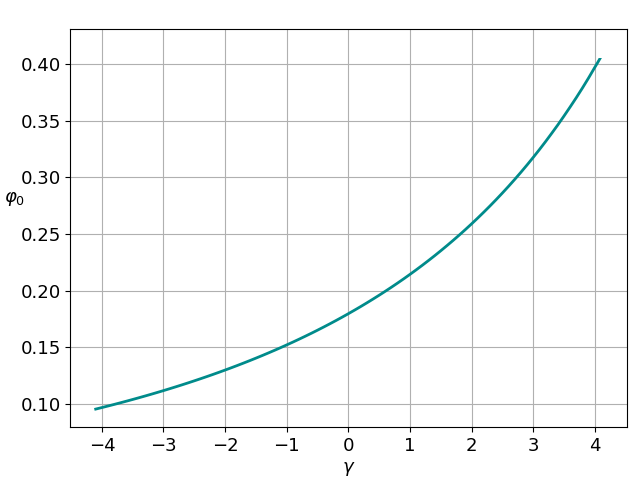
\includegraphics[scale=0.36]{oscillating_phi0_0.png} }
\end{minipage}
\hspace{3.5cm}
\begin{minipage}[h]{0.2\linewidth}
\center{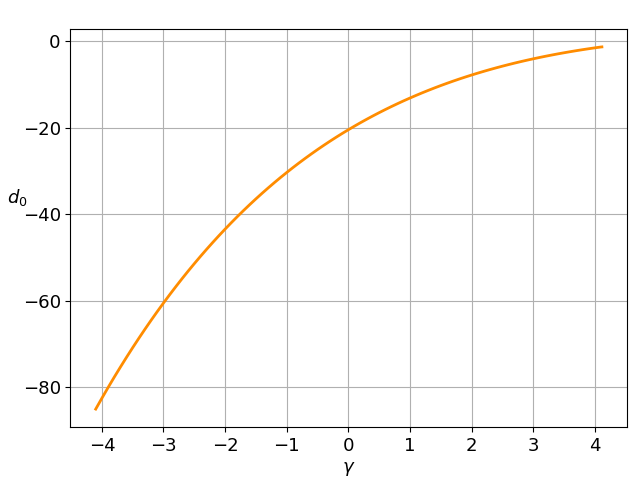
\includegraphics[scale=0.36]{oscillating_d0_0.png} }
\end{minipage}
\end{figure}

$$ x_0=0 $$

\end{frame}

\begin{frame}
\frametitle {Случай линейной краевой задачи с нелинейным отклонением }

$$ \phi_0 = - \operatorname{Re} \left( \frac{2 \mu \ch \mu x_0}{\mu \ch \mu + \sh \mu - \alpha_c x_0 \sh \mu x_0} \right), $$

$$ d_0 = \operatorname{Re} \left( \frac{3 \beta \mu (\ch (\mu + 2\,\mbox{Re}\mu) x_0 + \ch (\mu + 2i\,\mbox{Im}\mu) x_0 + 2 \ch \overline{\mu} x_0)}{\mu \ch \mu + \sh \mu - \alpha_c x_0 \sh \mu x_0} \right). $$

\end{frame}

\begin{frame}
\frametitle { Графики $ \phi_0(\gamma), \; d_0(\gamma) $ }

\begin{figure}[h]
\hspace{-4cm}
\begin{minipage}[h]{0.2\linewidth}
\center{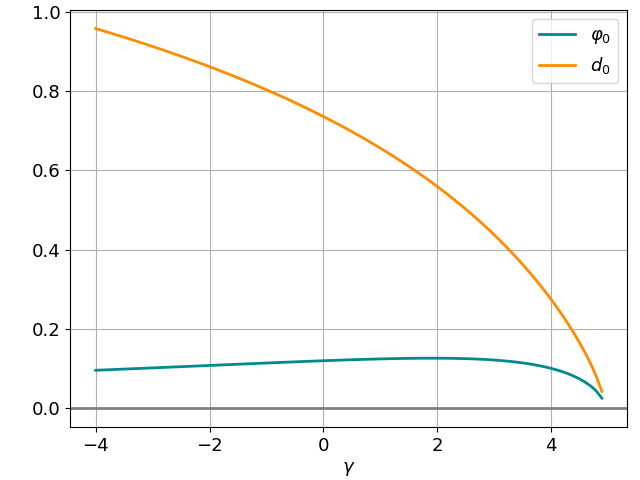
\includegraphics[scale=0.36]{oscillating_phi0d0_13_beta_minus.png} \\ a) $ \beta = -1.0 $ }
\end{minipage}
\hspace{3.5cm}
\begin{minipage}[h]{0.2\linewidth}
\center{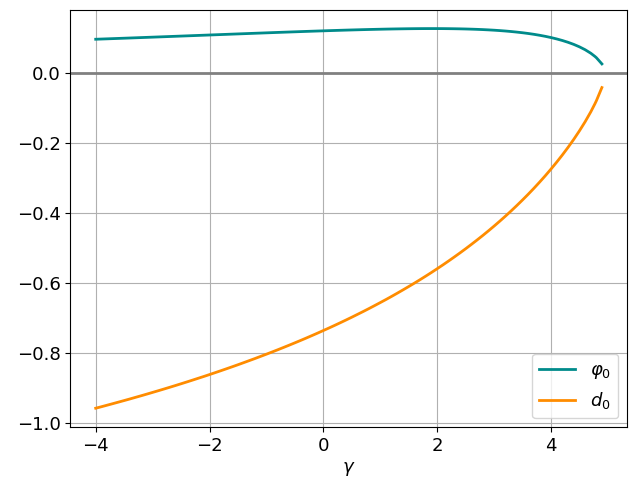
\includegraphics[scale=0.36]{oscillating_phi0d0_13_beta_plus.png} \\ b) $ \beta = 1.0 $ }
\end{minipage}
\end{figure}

$$ x_0=0.33 $$

\end{frame}

\begin{frame}
\frametitle{ Заключение }

\begin{itemize}
\item Для нелинейной динамической системы с импульсными воздействиями выделены области параметров, с разными бифуркационными сценариями. В каждой области изучены перестройки, происходящие в фазовом пространстве модельного отображения.

\vfill

\item Для краевой задачи со специальными краевыми условиями найдены критические значения параметров, при которых происходит потеря устойчивости нулевого решения. При значениях параметров близких к критическим на основе нормальной формы были определены условия появления неоднородных состояний равновесия и циклов. 
\end{itemize}

\end{frame}

\begin{frame}
\frametitle{ Значимость проведенных исследований }

\begin{block}{}
Полученные результаты могут быть использованы в области нелинейной динамики, математической биологии и теоретической физики. Дополнительно найденные устойчивые режимы нелинейной динамической системы с импульсными воздействиями могут быть использованы при моделировании ассоциативной памяти компьютера. Анализ устойчивости нулевого решения краевой задачи со специальными краевыми условиями позволит модифицировать некоторые модели популяции живых существ.
\end{block}

\end{frame}

\begin{frame}
\frametitle{ Список работ, опубликованных аспирантом }

\begin{enumerate}

\begin{scriptsize}
\item Ивановский Л.И., Самсонов С.О. Фазовые перестройки одной двумерной динамической системы с импульсным воздействием / Л.И. Ивановский, С.О. Самсонов // Модел. и анализ информ. систем. - 2014. - Т. 21, \textnumero~6. - С. 179-181.
\item Ivanovsky L.I. Stable regimes of dynamic systems with impulsive influences / L.I. Ivanovsky // 
Lobachevskii Journal of Mathematics. - 2017. - Vol. 38, No. 5. - P. 921-925.
\item Ивановский Л.И., Самсонов С.О. Динамика одного двумерного отображения и устойчивые режимы сингулярно возмущенной системы нейронного типа / Л.И. Ивановский, С.О. Самсонов // Вычисл. техн. в естеств. науках. Методы суперкомп. модел. - 2015. - \textnumero~2. - С. 121-132.
\item Ивановский Л.И. Динамические свойства одного класса импульсным систем / Л.И. Ивановский // Вычисл. техн. в естеств. науках. Методы суперкомп. модел. - 2015. - \textnumero~3. - С. 126-131.
\item Ивановский Л.И. Устойчивые режимы динамических систем с импульсными воздействиями / Л.И. Ивановский  // Динамические системы. - 2016. - Т. 6 (34), \textnumero~2. - С. 113-132.
\item Ивановский Л.И. Устойчивые режимы одного класса динамических систем с импульсными воздействиями / Л.И. Ивановский  // Вычисл. техн. в естеств. науках. Методы суперкомп. модел. - 2017. - \textnumero~4. - С. 35-42.
\end{scriptsize}

\end{enumerate}

\end{frame}

\begin{frame}
\frametitle{Свидетельства о государственной регистрации}

\begin{figure}[h]
\hspace{-3.2cm}
\begin{minipage}[h]{0.2\linewidth}
\center{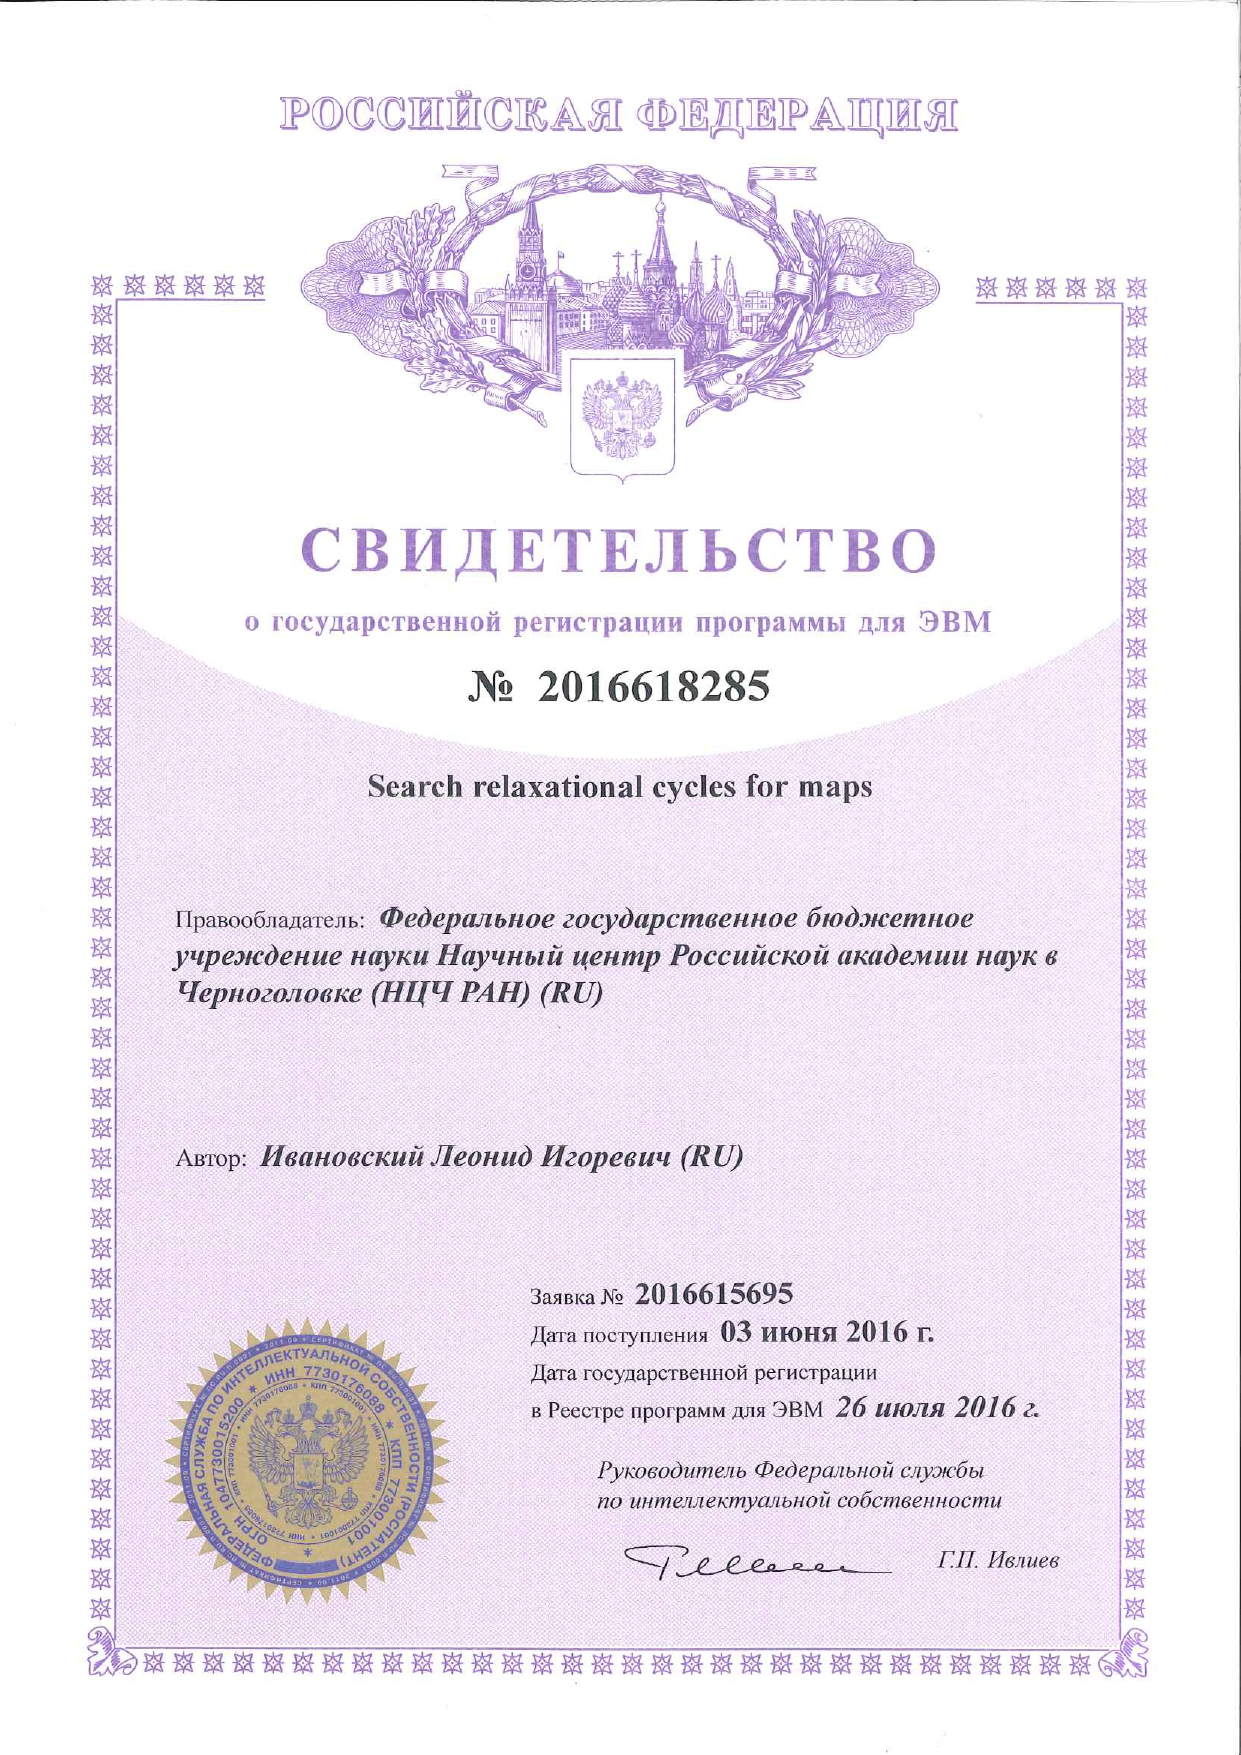
\includegraphics[scale=0.26]{2016618285.jpg} }
\end{minipage}
\hspace{3.2cm}
\begin{minipage}[h]{0.2\linewidth}
\center{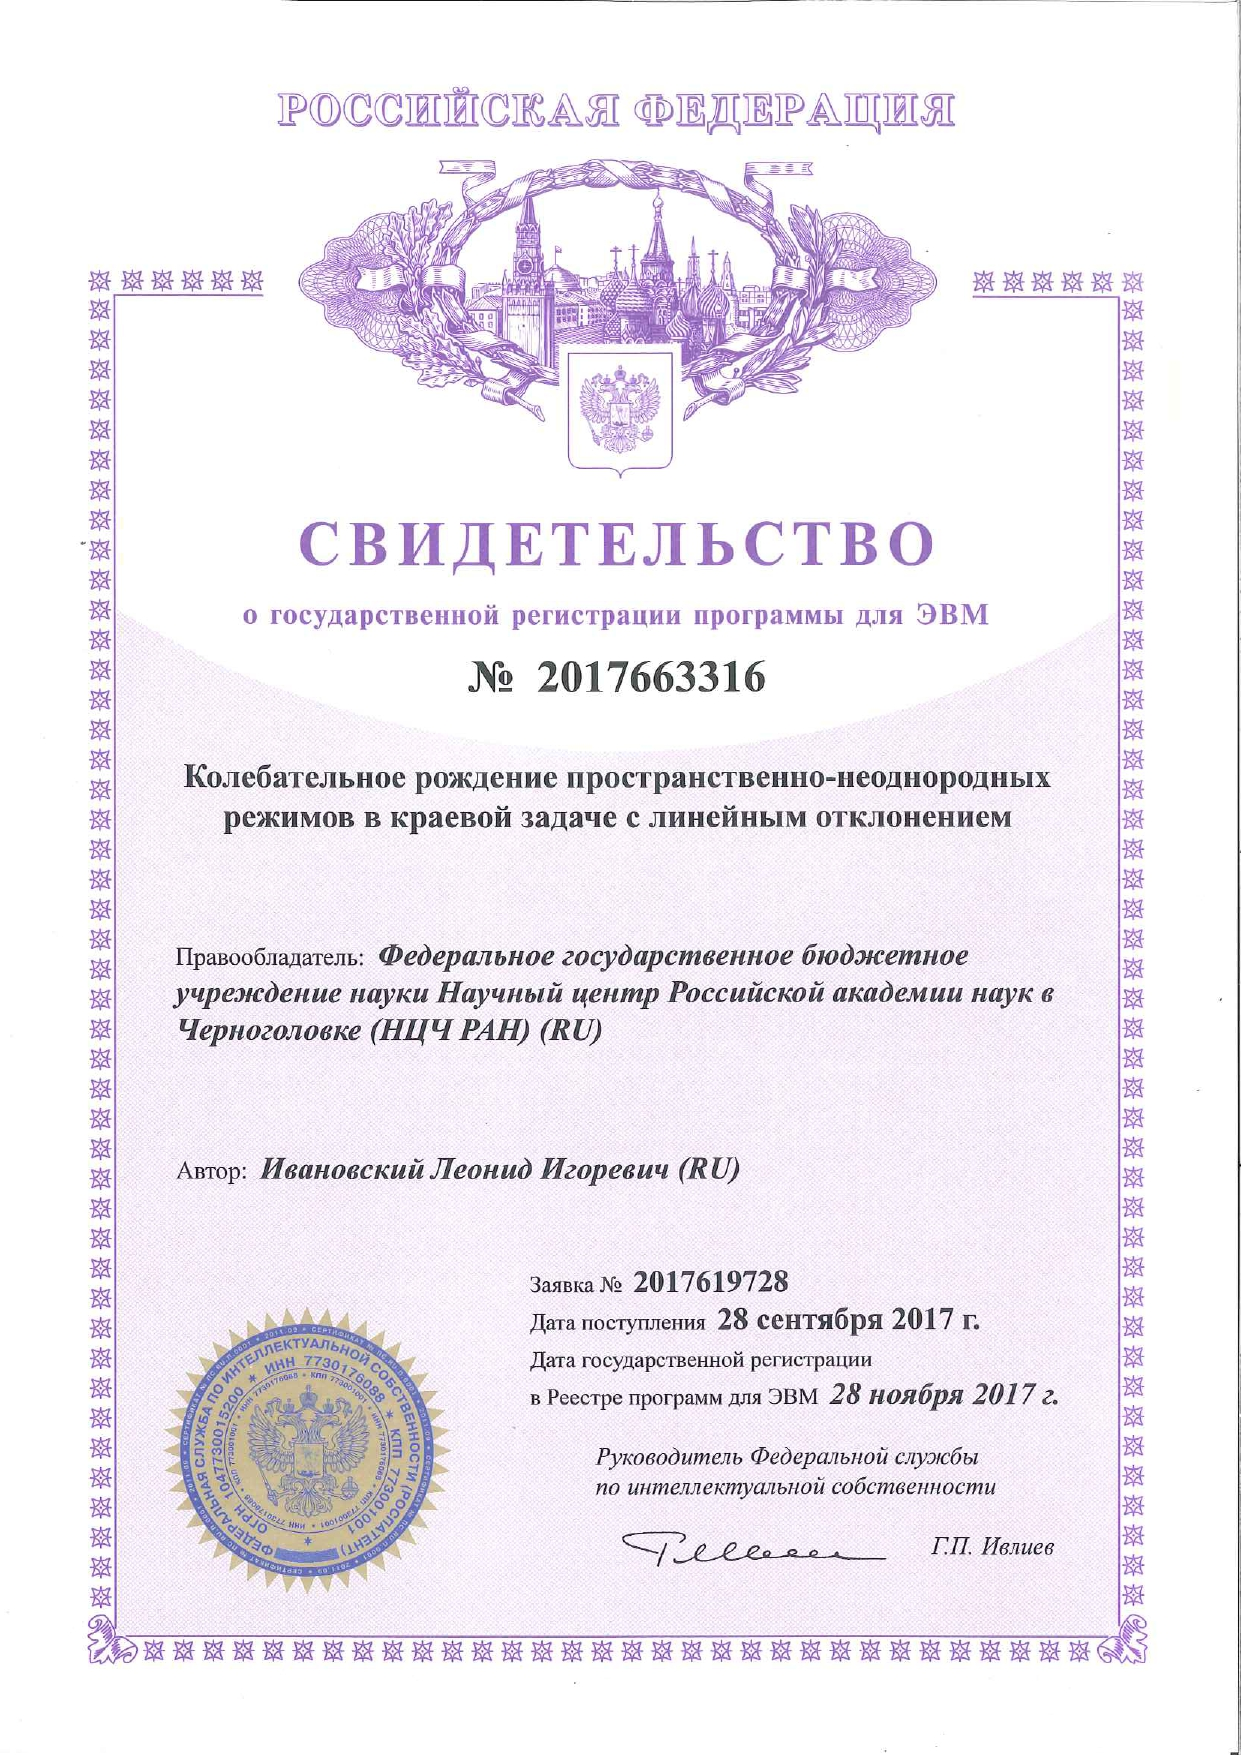
\includegraphics[scale=0.26]{2017663316.jpg} }
\end{minipage}
\end{figure}

\end{frame}

\begin{frame}[plain]
\maketitle
\small
\begin{tabular}[t]{@{}l@{\hspace{3pt}}p{.29\textwidth}@{}}
Аспирант: & \\
Ивановский Л.И.
\end{tabular}%
\small
\begin{tabular}[t]{@{}l@{\hspace{3pt}}p{.3\textwidth}@{}}
Научный руководитель: & \\
д. ф.-м.н., профессор Глызин С.Д.
\end{tabular}%
\end{frame}

\end{document}
